\section{Results}

The model has been tested in a series of benchmark environments, each with a different number of arms and reward distributions. The performance has been compared with the following algorithms: Random Baseline, Upper-Confidence Bound (UCB), Thompson Sampling, and Epsilon-Greedy. The results are
summarized in table \ref{fig:perf_plot}.

% Description of the environments
\subsection{Game variants}
\noindent The game environments considered in this work are non-stationary K-Armed Bandits with Binomial rewards. In particular, the agent is evaluated over a number $T_{\text{trials}}$ of \textit{trials}, each composed by an arbitrary number $T_{\text{rounds}}$ of \textit{rounds}; each \textit{trial} is characterized by a different reward distribution $\mathbf{p}\sim\mathcal{U}(0,1)^{K}$ (although in practice the bounds have been set to $(0.1, 0.9)$ such that the distributions are less trivial). Our goal in this work is to investigate the performance of the agent in a non-stationary environment with Binomial reward distributions, meaning that its underlying distribution changes over time.
We choose this setting as it resembles an ecological scenario in which an animal has to forage in a patchy environment, where the reward of a given patch can change over time.
More specifically, we used four different variants:

\noindent \textbf{Zero-steps distribution shift} [\textsc{KAB-0}]: the reward distribution changes immediately at the end of a trial $i$ to a new one $i+1$ as $\mathbf{\omega}_{i} \to \mathbf{\omega}_{i+1}$.

\noindent \textbf{Epsilon-steps distribution shift} [\textsc{KAB-$\epsilon$}]: the reward distribution $\omega$ changes gradually over rounds, tracked as time $t$, such that its shape tends towards a target distribution $\bar{\omega}_{i}$ as
$\tau_{\omega}\dot{\omega}_{t}=\bar{\omega}_{i}-\omega_{t}$. Once distance is below a threshold $\epsilon$ as $\vert \bar{\omega}_{i} - \omega_{t}\vert < \epsilon$, the target distribution is changed to a new one $\bar{\omega}_{i}\to\bar{\omega}_{i+1}$.

\noindent \textbf{Sinusoidal distribution shift} [\textsc{KAB-$\sin$}]: the reward distribution changes over rounds, with the probability of each arm following a sine wave with a specific frequency $f_{k}$ and amplitude $1$. At any given time $t$, the distribution is $\omega_{t}=\{\sin(2\pi f_{k}
t)\text{  for }k=1\ldots K\}$ and it is
normalized as $\omega_{t} = \omega_{t}(\sum_{k} \omega_{t,i})^{-1}$ such that it sums to $1$.

\noindent \textbf{Partial sinusoidal distribution shift} [\textsc{KAB-$\sin$P}]: identical to the sinusoidal distribution shift, but only a subset of the arms changes sinusoidally while the rest is kept at a constant value.


% Results: scores and brief discussion
\subsection{Performance comparison}

\begin{figure}[h]
    \centering
    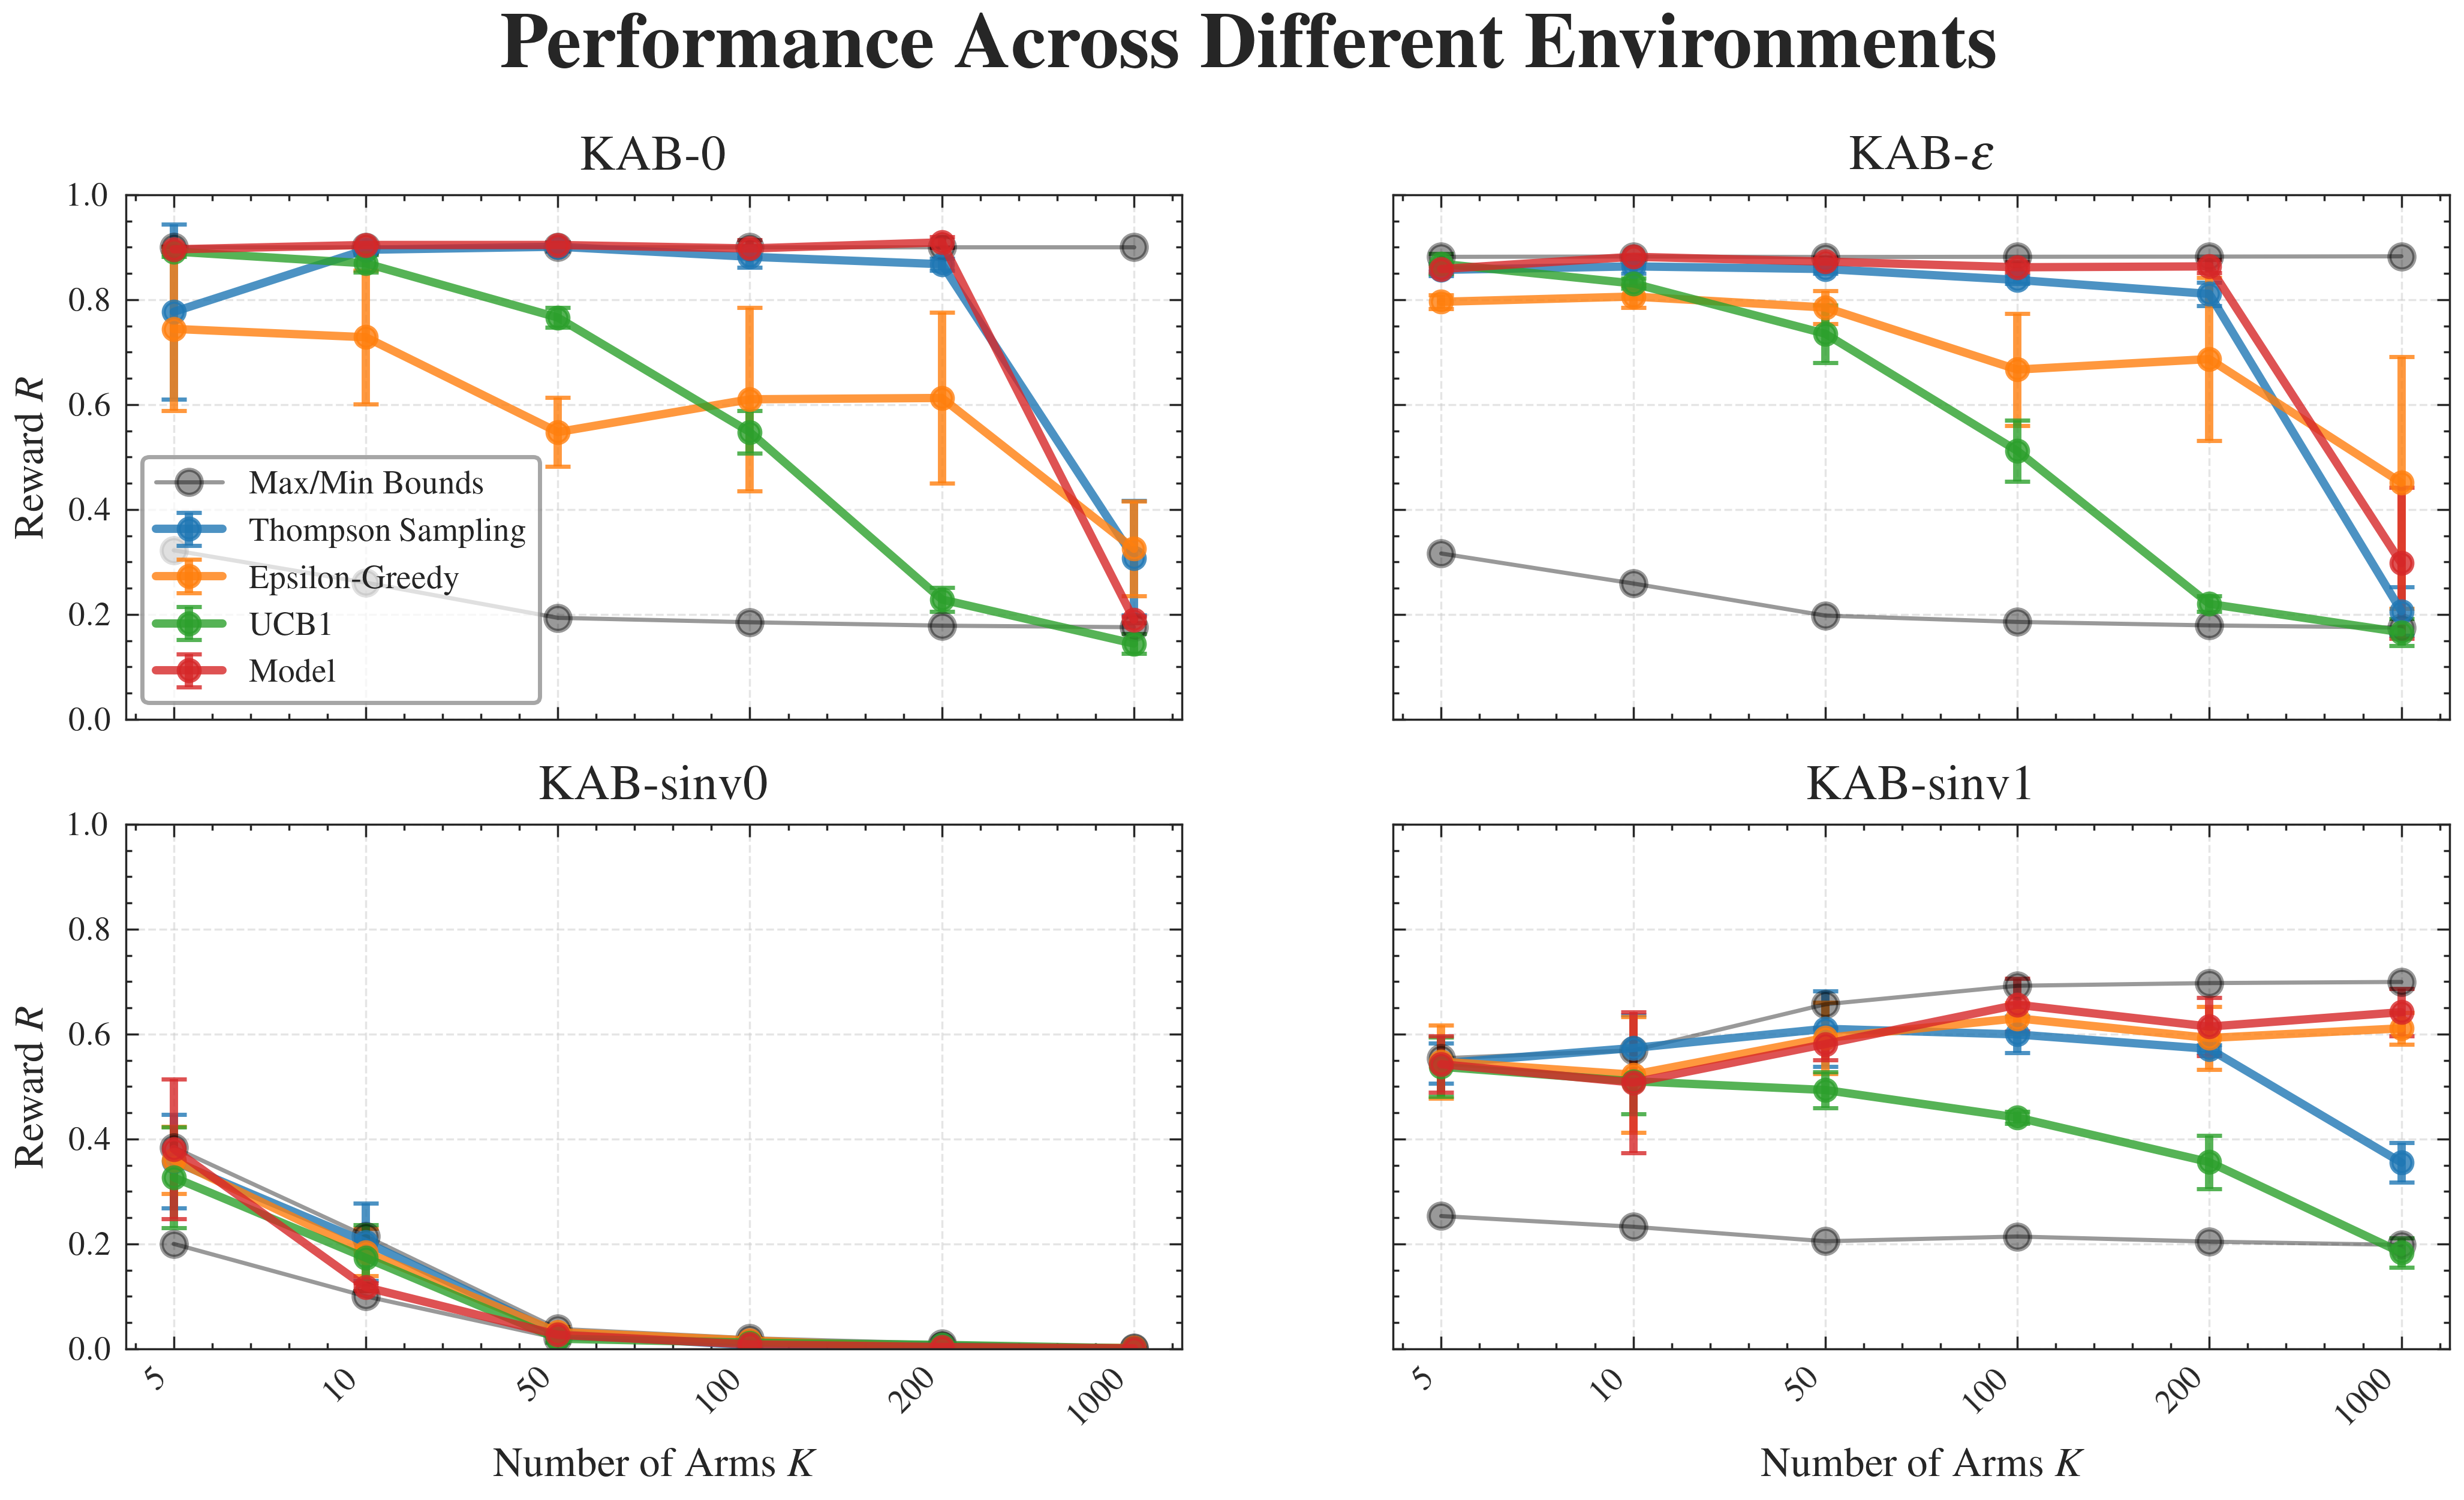
\includegraphics[width=1.\textwidth]{figures/performance_plot.png}
    \caption{\textsc{Performance comparison for different values of $K$ and game variants} \textit{The model is compared with Thompson Sampling, Epsilon-Greedy, and UCB. The performance is measured as the average reward obtained by the agent over a number of trials.}}
    \label{fig:perf_plot}
\end{figure}

\subsection{Decision-making dynamics}

\noindent For a better understanding of the qualitative differences between the models, we analyzed the progress over the rounds and tracked the selected arms in the simplest case of zero-steps distribution shift. Additionally, in order to quantify the variability of the decision policy at a given time and highlight the particularity of each
decision-making behaviour, we calculated the entropy of the distribution of chosen
arms over a time window of 20 rounds as $H=-\sum^{K}_{i} p_{i}\log(p_{i})$. In figure \ref{fig:entropy_fig1}, it is plotted for each model the raster plot of selected arms together with its level of entropy. As expected, the over shape of the changes in the entropy over time are rather specific to
each model. In particular, the UCB algorithm showed the highest variability, marked by a persistent exploratory behaviour throughout the trials despited converging to reward options. Thompson Sampling was able to reach most solutions, although with difficulty in adapting to new reward distributions
leading to high entropy levels.
$\epsilon-$Greedy also showed a good performance quite reliably, with the greedy strategy assuring low entropy for most of the rounds.
Similar behaviour was observed for our model, which was able to reach the optimal policy and maintain it over time, with entropy peaking mostly at the beggining of the trials and being, on average, the lowest among all models.
Indeed, the model dynamics make it particularly suited for the task of non-stationary K-armed bandits, as it is able to quickly adapt to new reward distributions and firmly maintain a greedy policy.

\begin{figure}[h]
    \centering
    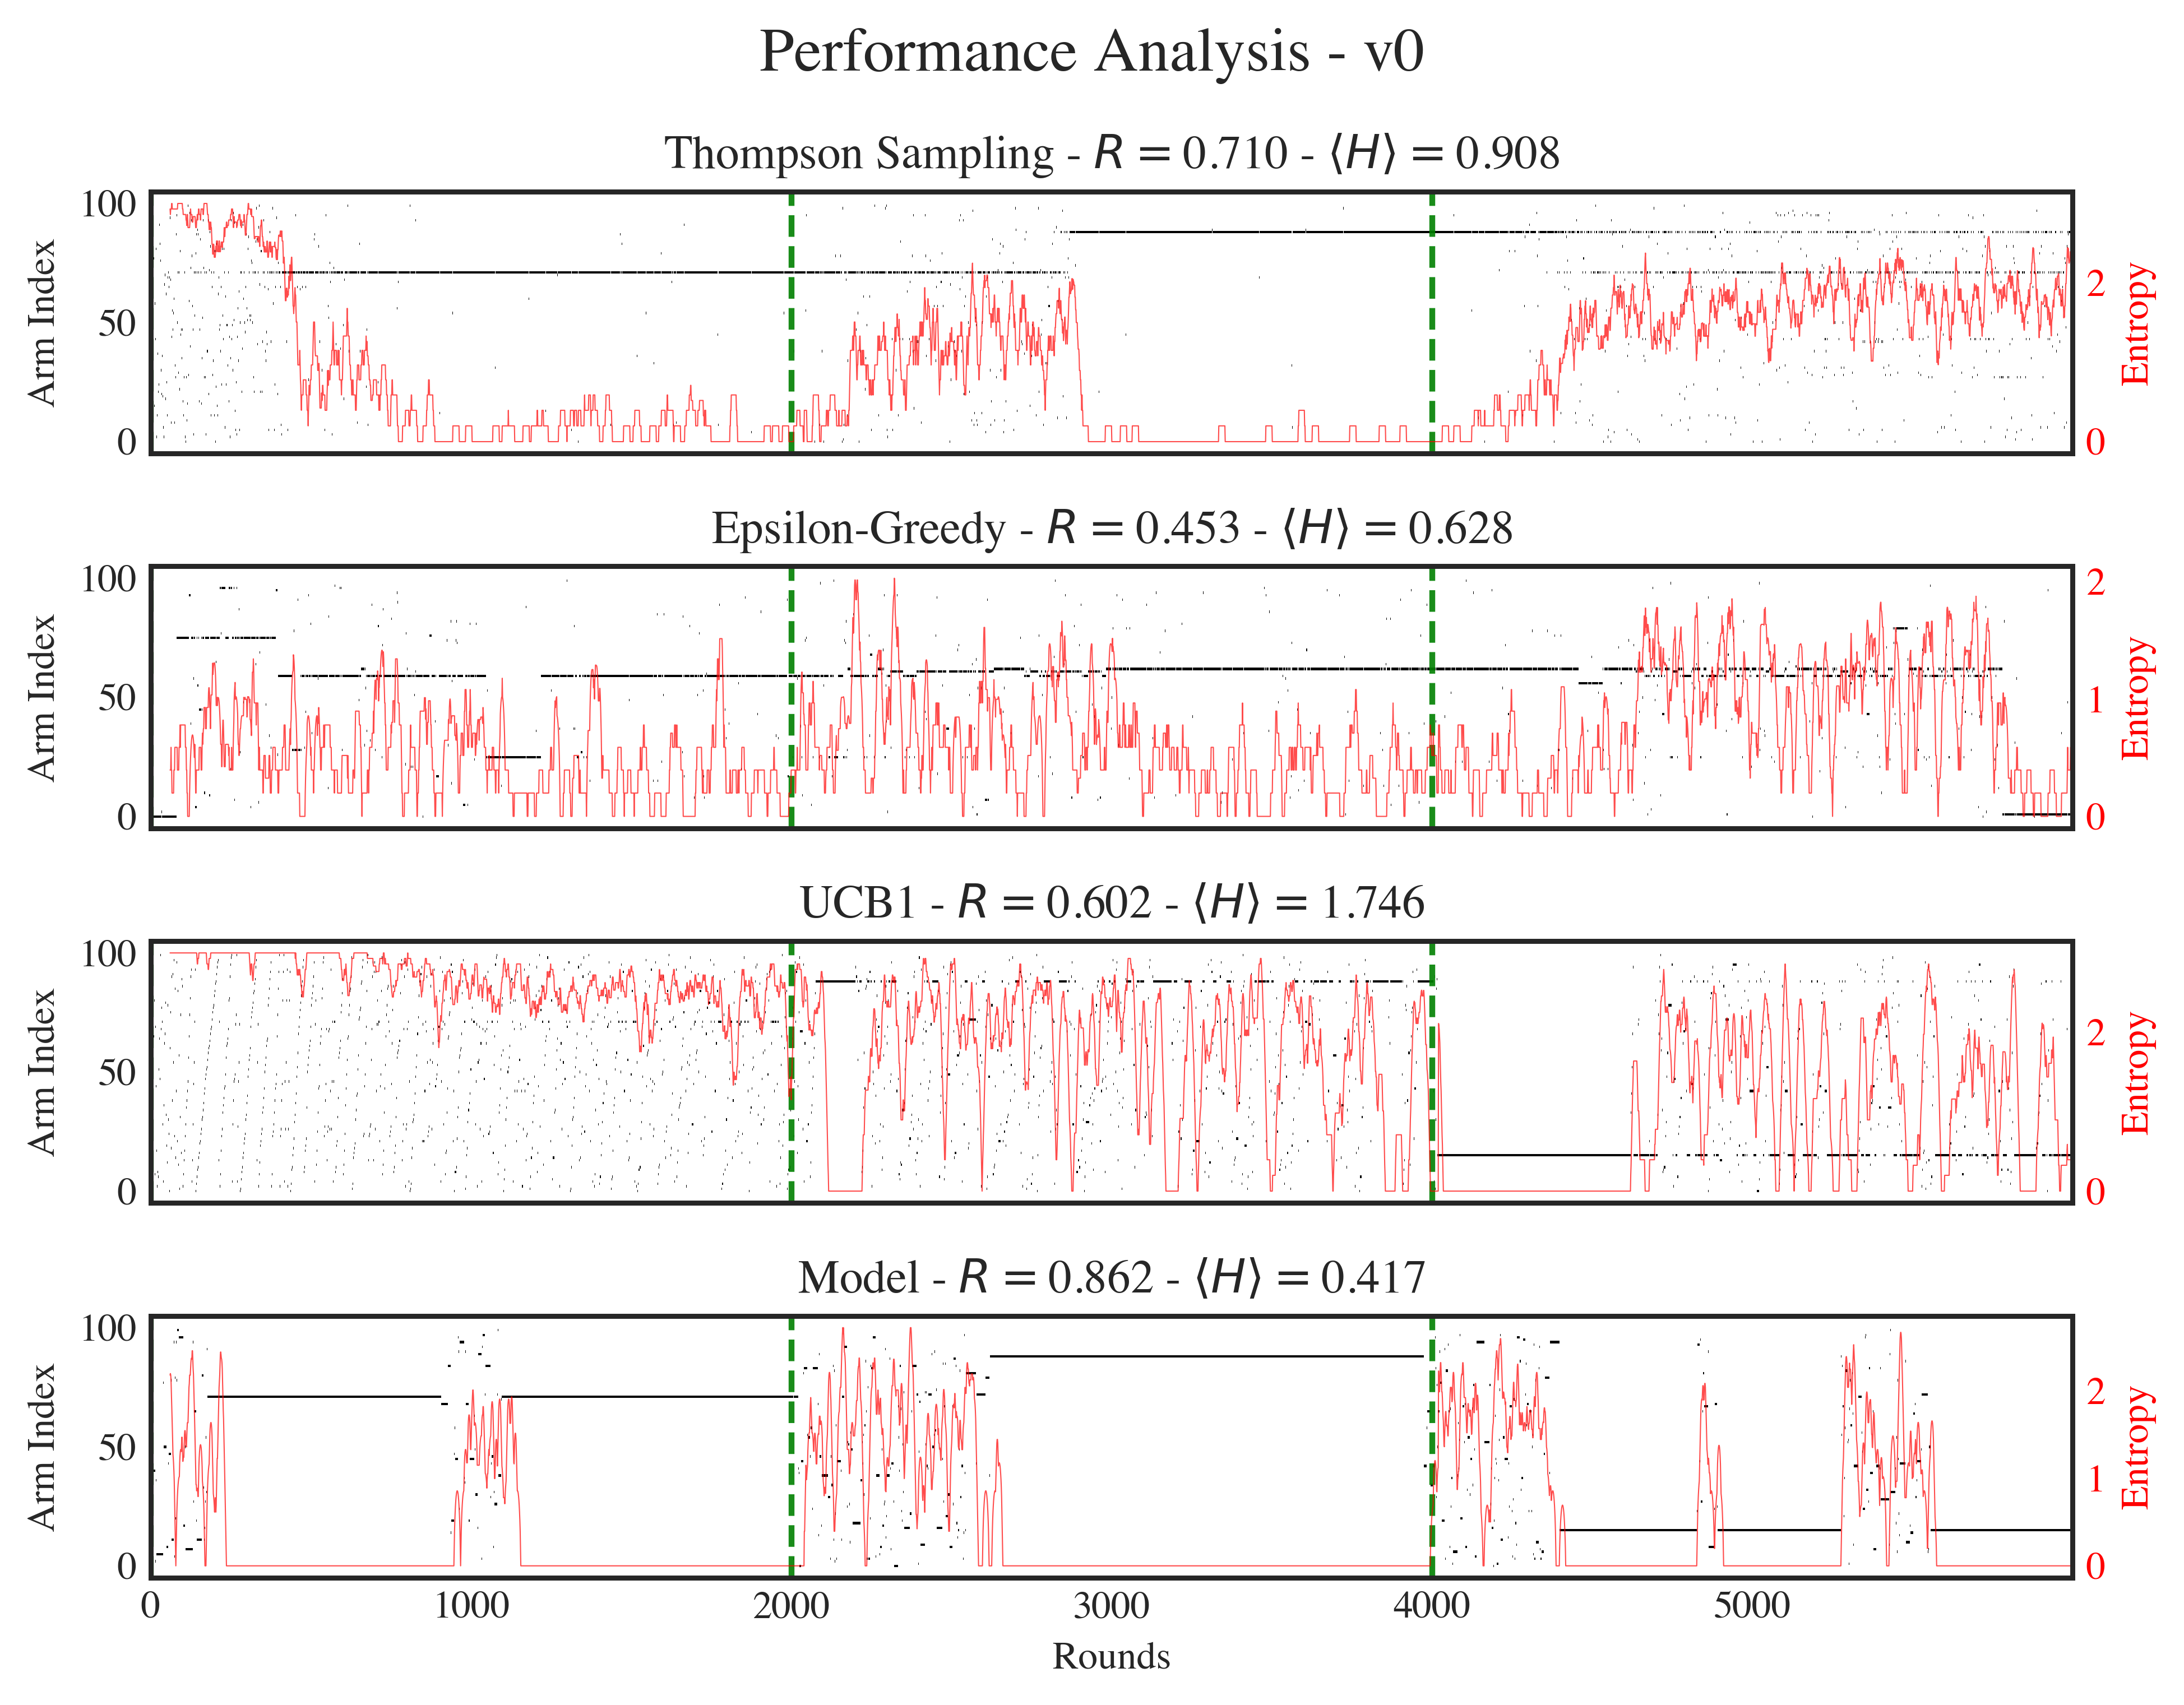
\includegraphics[width=1.0\textwidth]{figures/performance_analysis_KABv0.png}
    \caption{\textsc{Decision-making dynamics for different models} \textit{The raster plot shows the selected arms over time (black dots), while the entropy plot shows the variability of the decision policy (red lines). It is also reported the total reward and average entropy over all trials.}}
    \label{fig:entropy_fig1}
\end{figure}




\subsection{Robustness and parameter sensitivity}


